%
% Class document definition
%
\documentclass[msc]{template/ppgccufmg}  % [phd] | [msc]



%
% Document used packages
%
\usepackage[brazil]{babel}
\usepackage[utf8]{inputenc}
\usepackage[T1]{fontenc}
\usepackage{type1ec}
\usepackage{graphicx}
\usepackage[a4paper,
      portuguese,
      bookmarks=true,
      bookmarksnumbered=true,
      linktocpage,
      colorlinks,
      citecolor=black,
      urlcolor=black,
      linkcolor=black,
      filecolor=black,
]{hyperref}
\usepackage[square]{natbib}
\usepackage{multirow}
\usepackage[usenames,dvipsnames]{xcolor} 


\hyphenation{re-qui-si-to}

\sloppy



%
% The document body and structure
%
\begin{document}



% Definitions for ppgccufmg class
\ppgccufmg{
    title={Grafos como uma primitiva do plano de controle para análise e 
        gerenciamento de Redes Definidas por Software},
    authorrev={Pantuza, Gustavo},
    cutter={M1234x}, % INFORMAÇÃO QUE VAI NA FICHA CATALOGRÁFICA
    cdu={100.0*01.10},  % Define o identificador CDU do documento, fornecido pela Secretaria do Curso.
    university={Universidade Federal de Minas Gerais},
    course={Ciência da Computação},
    address={Belo Horizonte},
    date={2015-03},
    keywords={Redes definidas por software, Openflow, Grafos, 
        Gerenciamento de redes, Sistemas distribuídos, Redes de computadores},
    advisor={Luiz Filipe Menezes Vieira},
    abstract=[brazil]{Resumo}{src/abstract_pt},
    abstract=[english]{Abstract}{src/abstract_en},
    %abstract=[brazil]{Resumo Estendido}{resumoest}, %resumoest.tex
    %dedication={dedicatoria},
    %ack={agradecimentos},
    %  ack=[Acknowledgments]{ack},
    epigraphtext={Live long and prosper!}{Mr. Spock},
}




% Chapters and files that compose the document content
%
% Introduction
%
\section{Introdução}


%
% Community emvolvment
%
\begin{frame}\frametitle{Apresentação}

	\begin{figure}[h]
        \centering
        
\includegraphics[scale=0.5]{images/community.png}
    \end{figure}
\end{frame}


%
% Motivation
%
\begin{frame}\frametitle{Motivação}
   
    \begin{itemize}
        \setlength{\itemsep}{1cm}
        \item A Internet demanda que a infraestrutura evolua em paralelo com 
            as aplicações e serviços
        \item Algoritmos em grafos são base para diversas aplicações em rede
        \item Computação feita em diferentes nós da rede repetidamente
        \item Logicamente centralizado, o plano de controle permite 
            minimizar a quantidade de computações
    \end{itemize}
\end{frame}


%
% Problem
%
\begin{frame}\frametitle{Problema}
    \begin{itemize}
        \setlength{\itemsep}{1cm}
        \item Uma visão topológica global é um dos principais aspectos do 
              paradigma das Redes definidas por software.
        \item Grafos representam de maneira natural e precisa a topologia 
            de uma rede.
        \item Grafos deveriam ser um recurso básico, uma premissa em 
            controladores SDN
    \end{itemize} 
\end{frame}


%
% Scientific contributions
%
\begin{frame}\frametitle{Contribuições científicas}
    \begin{itemize}
        \setlength{\itemsep}{1cm}
        \item Uma abstração da rede na forma de um grafo dinamicamente 
            atualizado.
        \item Avaliações do controlador, da rede e do protocolo OpenFlow
        \item Avaliação de grafos como primitiva em SDN
    \end{itemize}
\end{frame}


\section{Fundamentação teórica}

\section{SDN}



%
% SDN
%
\begin{frame}\frametitle{SDN}

    \begin{itemize}
    \item SDN é apenas um modelo
    \vspace*{0.5cm}
    \item Um \emph{design} para construção e administração de redes
    \vspace*{0.5cm}
    \item A separação dos planos de controle e de dados torna o 
          funcionamento da rede mais flexível
    \end{itemize}
\end{frame}

%
% SDN
%
\begin{frame}\frametitle{Características}

    \begin{itemize}
    \item Torna a rede programável
    \vspace*{0.1cm}
    \item Flexibilidade na administração da rede
    \vspace*{0.1cm}
    \item Controle logicamente centralizado
    \vspace*{0.1cm}
    \item Configurável via programação
    \vspace*{0.1cm}
    \item Padronização aberta 
    \end{itemize}
\end{frame}


%
% Openflow
%
\begin{frame}\frametitle{Openflow}

    \begin{itemize}
    \item Se SDN é só um modelo, como implementá-lo?
    \end{itemize}
    	\begin{figure}[h]
        \centering
        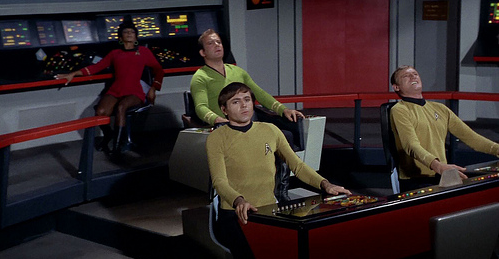
\includegraphics[scale=0.5]{images/control-room.png}
    \end{figure}
\end{frame}



%
% Openflow
%
\begin{frame}\frametitle{Openflow}

    \begin{itemize}
    \item Openflow é um protocolo que possibilita experimentos e aplicações
          em SDN
    \end{itemize}
    	\begin{figure}[h]
        \centering
        
\includegraphics[scale=0.3]{images/openflow.png}
    \end{figure}
\end{frame}


%
% Openflow
%
\begin{frame}\frametitle{Openflow}

    \begin{itemize}
    \item \href{http://archive.openflow.org/documents/openflow-wp-latest.pdf}{Artigo} publicado em 2008 
    \item Permitiu que pesquisadores pudessem criar experimentos com novos
          protocolos em redes convencionais 
    \end{itemize}

\end{frame}




%
% Openflow
%
\begin{frame}\frametitle{Porque é tão importante?}

    \begin{itemize}
    \item A arquitetura da Internet tem deficiências
    \item Inovações em rede custam caro
    \item A arquitetura continua acoplada à infraestrutura
    \item O Openflow define um padrão que qualquer fabricante de     
          \emph{hardware} de rede pode implementar
    \end{itemize}

\end{frame}


\subsection{O protocolo OpenFlow}


%
% Openflow
%
\begin{frame}\frametitle{Openflow}

    \begin{itemize}
    \item Openflow é um protocolo que possibilita experimentos e aplicações
          em SDN
    \end{itemize}
    \begin{figure}[h]
        \centering
        
\includegraphics[scale=0.2]{images/openflow}
    \end{figure}
\end{frame}


%
% Openflow
%
\begin{frame}\frametitle{Openflow}

    \begin{itemize}
        \setlength{\itemsep}{.5cm}
    \item \href{http://archive.openflow.org/documents/openflow-wp-latest.pdf}
        {OpenFlow: Enabling Innovation in Campus Networks} publicado em 2008 
    \item Permitiu que pesquisadores criassem experimentos com novos
          protocolos em redes convencionais.
    \end{itemize}

\end{frame}




%
% Openflow
%
\begin{frame}\frametitle{Definição}

    \begin{itemize}
        \setlength{\itemsep}{.5cm}
        \item Consiste em uma interface de programação para o \emph{switch}
        \item A interface separa de maneira clara os planos de dados e de 
            controle
        \item Um programador pode, através de um programa, controlar a
            forma como um \emph{switch} executa seu encaminhamento de pacotes
        \item O OpenFlow foi criado como um padrão aberto
    \end{itemize}
\end{frame}


%
% Openflow
%
\begin{frame}\frametitle{Componentes}
    Na arquitetura estabelecida pelo protocolo OpenFlow existem dois papéis
    principais.

    \begin{figure}[h]
        \centering
        
\includegraphics{images/controller-secure-switch}
        \caption{Da esquerda pra direita, plano de controle e plano de dados}
    \end{figure}

\end{frame}


%
% Openflow
%
\begin{frame}\frametitle{Arquitetura OpenFlow}

    \begin{figure}[h!]
        \centering
        \label{fig:switch-arch}
        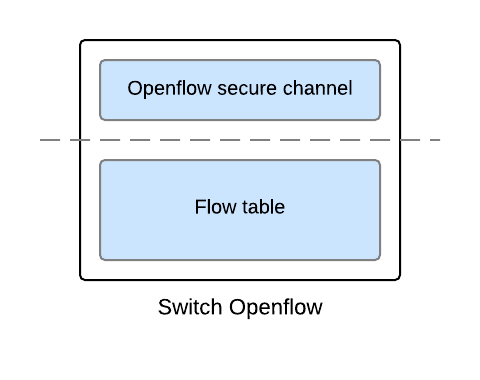
\includegraphics[width=\linewidth]{images/switch-architecture}
        \caption{Arquitetura do comutador OpenFlow}
    \end{figure}

\end{frame}



%
% Switch Archtecture
%
\begin{frame}\frametitle{Arquitetura Openflow}

    \begin{itemize}
        \setlength{\itemsep}{.5cm}
    \item \textbf{Canal seguro OpenFlow}: É a conexão segura entre o
          controlador e o switch openflow
    \item \textbf{Tabela de fluxos}: É a tabela onde são identificados os fluxos
    \item Para cada fluxo tem-se uma ação (action) a ser tomada
    \end{itemize}
\end{frame}


%
% Switch Archtecture
%
\begin{frame}\frametitle{Tabela de fluxos}
    \begin{table}[h!]
    \small
    \centering
    \begin{tabular}{ | l | l | l | l |}
    \hline
    \textbf{Cabeçalho} & \textbf{Contadores} & \textbf{Ações} &
    \textbf{Prioridade} 
    \\ \hline porta de ingresso=5 & 55635 bytes & \pbox{20cm}{Encaminhar 
    \\ porta=8} 
    & 100 \\ \hline
    \pbox{20cm}{Endereço ip=192.168.1.42 \\ porta=80} & 4032 bytes &
    \pbox{30cm}{Rescrita \\ ip=192.168.1.100} & 500 \\ 
    \hline Protocolo IP=UDP & 100 bytes 
    & Drop & 700 \\ \hline
    \end{tabular}
    \caption{Tabela de fluxos simplificada}
    \label{tbl:flowtable}
\end{table}

\end{frame}

%
% Switch Archtecture
%
\begin{frame}\frametitle{Cabeçalho OpenFlow}

    \begin{itemize}
    \item Um fluxo é identificado pelos seguintes campos do cabeçalho 
          Openflow:
    \end{itemize}
	\begin{figure}[h]\hspace*{-1.2cm}
        \centering
        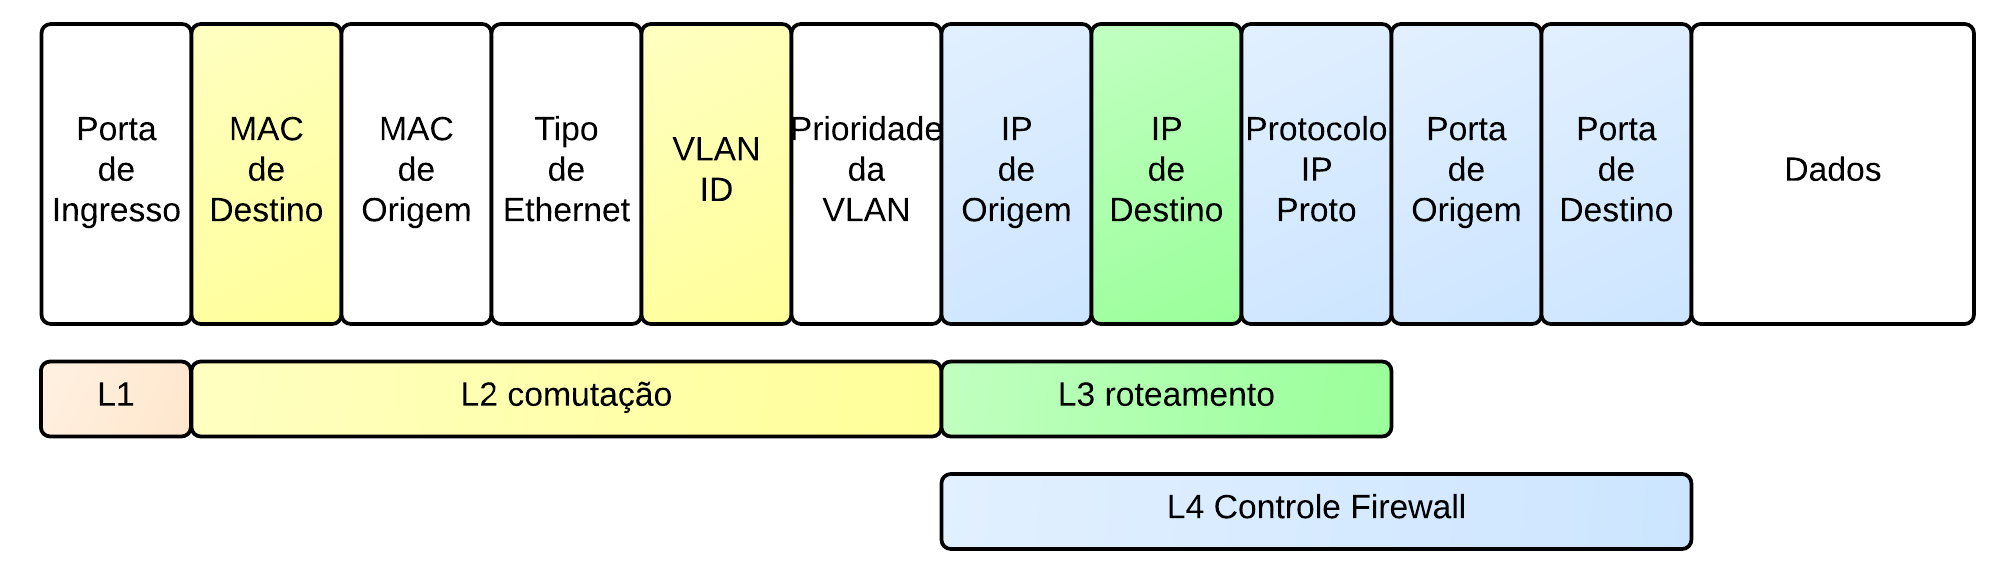
\includegraphics[width=\linewidth]{images/openflow-header}
    \end{figure}
\end{frame}



%
% Actions
%
\begin{frame}\frametitle{Ações}

	\begin{figure}[h]
        \centering
        
\includegraphics[scale=0.5]{images/action.png}
    \end{figure}
    
\end{frame}


%
% Actions
%
\begin{frame}\frametitle{Tipos de ações}

    \begin{columns}[T] % align columns
        \begin{column}{.33\textwidth}

            \begin{itemize}
                \item Forwarding
                \item Drop
                \item Set
                \item strip
                \item Copy-in
                \item Copy-out
                \item Push
                \item Pop
                \item Dec
            \end{itemize}
        \end{column}%
        \hfill%
        \begin{column}{.67\textwidth}
            \begin{figure}[!htb]
                \centering
                
\includegraphics[scale=0.5]{images/action-types}
            \end{figure}
        \end{column}%
    \end{columns}

\end{frame}


%
% Controller
%
\begin{frame}\frametitle{Controlador}

    \begin{itemize}
        \setlength{\itemsep}{.5cm}
    \item É um software que se conecta de maneira segura ao switch openflow
          com o objetivo de manipular sua tabela de fluxos
    \item Esse software pode ser distribuído
    \item Ele representa uma entidade lógica e centralizada
    \item Permite que outros programas troquem mensagens com o 
        plano de controle da rede
    \item Pode calcular estatísticas da rede
    \end{itemize}

\end{frame}


%
% Controller
%
\begin{frame}\frametitle{Controlador}

    \begin{itemize}
    \item Cabe ao programador lidar com os problemas típicos em 
          desenvolvimento de software:
          \begin{itemize}
          \item Tolerância a falha
          \item Persistência
          \item Eficiência
          \item Projeto/design de implementação
          \item debugging
          \item Testes
          \end{itemize}
    \end{itemize}
\end{frame}


%
% Controller
%
\begin{frame}\frametitle{Controlador}

    \begin{itemize}
    \item Controladores Openflow:
          \begin{itemize}
          \item Biblioteca \href{http://opennetworkingfoundation.github.io/libfluid/index.html}{Libfluid}
                para criação de aplicações/controladores em SDN
          \item \href{http://www.noxrepo.org/nox/about-nox/}{Nox Controller}
          \item \href{https://openflow.stanford.edu/display/Beacon/Home}{Beacon}
          \item \href{http://www.noxrepo.org/pox/about-pox/}{Pox Controller}
          \item \href{http://osrg.github.io/ryu/}{Ryu}
          \end{itemize}
    \end{itemize}
\end{frame}

\section{architecture}


%
% Archtecture
%
\begin{frame}\frametitle{Arquitetura Openflow}

    \begin{itemize}
    \item Temos dois papeis principais:
        \begin{itemize}
        \item Controlador
        \item Switch Openflow
        \end{itemize}
    \item Algo te lembra plano de dados e controle desacoplados?
    \end{itemize}
    
	\begin{figure}[h]
        \centering
        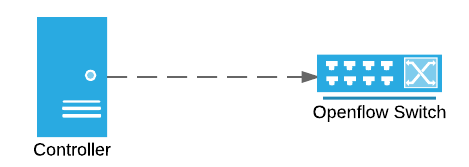
\includegraphics[scale=0.6]{images/controller-to-openflow.png}
    \end{figure}
\end{frame}



%
% Switch Archtecture
%
\begin{frame}\frametitle{Arquitetura do Switch Openflow}

    \begin{itemize}
    \item Internamente um Switch openflow é assim:
    \end{itemize}
    
	\begin{figure}[h]
        \centering
        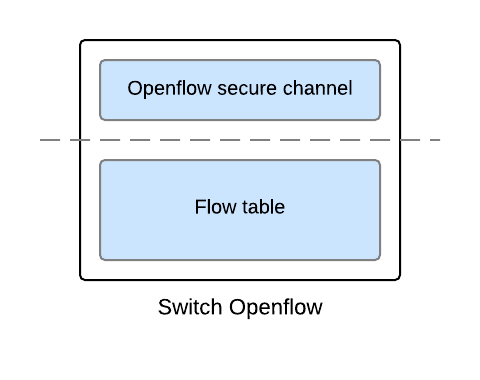
\includegraphics[scale=0.5]{images/openflow-switch-architecture.png}
    \end{figure}
\end{frame}

%
% Switch Archtecture
%
\begin{frame}\frametitle{Arquitetura Openflow}

    \begin{itemize}
    \item \textbf{Openflow secure channel}: É a conexão segura entre o
          controlador e o switch openflow
    \vspace*{0.5cm}
    \item \textbf{Flow table}: É a tabela onde são identificados os fluxos
    \vspace*{0.5cm}
    \item Para cada fluxo tem-se uma ação (action) a ser tomada
    \end{itemize}
\end{frame}

%
% Switch Archtecture
%
\begin{frame}\frametitle{Arquitetura Openflow}

    \begin{itemize}
    \item Um fluxo é identificado pelos seguintes campos do cabeçalho 
          Openflow:
    \end{itemize}
	\begin{figure}[h]\hspace*{-1.2cm}
        \centering
        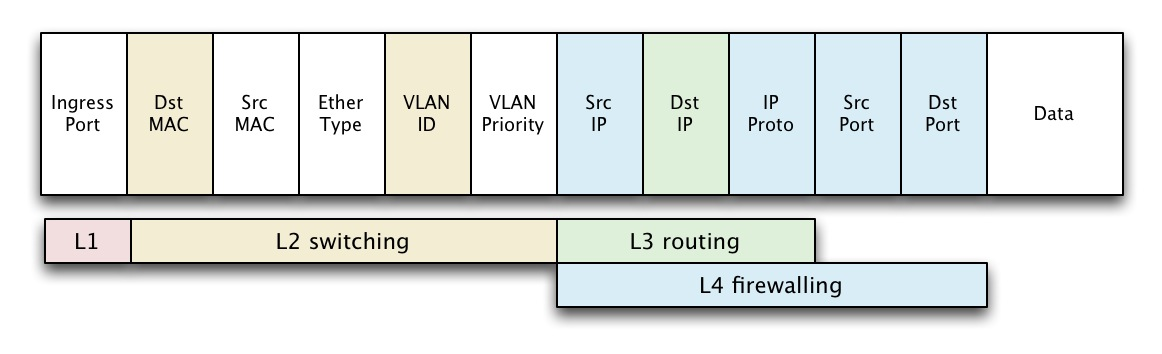
\includegraphics[scale=0.32]{images/openflow-header.jpg}
    \end{figure}
    
\end{frame}


%
% Actions
%
\begin{frame}\frametitle{Actions}

	\begin{figure}[h]
        \centering
        
\includegraphics[scale=0.5]{images/action.png}
    \end{figure}
    
\end{frame}


%
% Actions
%
\begin{frame}\frametitle{Tipos de Actions}

    \begin{itemize}
    \item Forwarding
    \item Drop
    \item Set
    \item strip
    \item Copy-in
    \item Copy-out
    \item Push
    \item Pop
    \item Dec
    \end{itemize}

\end{frame}


%
% Flow table 
%
\begin{frame}\frametitle{Tabela de Fluxos}

\begin{center}
    \begin{tabular}{ | l | l | l | l |}
    \hline
    \textbf{Header} & \textbf{Counters} & \textbf{Actions} & \textbf{Priority} \\ \hline
    in\_port=5 & 55635 bytes & \pbox{20cm}{Forward \\ port=8} & 100 \\ \hline
    \pbox{20cm}{ip=192.168.1.42 \\ port=80} & 4032 bytes & \pbox{30cm}{Set \\ rewrite \\ ip=192.168.1.100} & 500 \\ \hline
    ipproto=UDP & 100 bytes & Drop & 700 \\ \hline
    \end{tabular}
\end{center}

\end{frame}

%
% Controller
%
\begin{frame}\frametitle{Controlador}

    \begin{itemize}
    \item É um software que se conecta de maneira segura ao switch openflow
          com o objetivo de manipular sua tabela de fluxos
    \item Esse software pode ser distribuído
    \item Ele representa uma entidade lógica e centralizada
    \item É possível ter visão e controle de estado global da rede
    \item Permite que outros serviços e programas façam requisições e troca
          de mensagem com o plano de controle da rede
    \item Pode calcular estatísticas da rede
    
    \end{itemize}

\end{frame}


%
% Controller
%
\begin{frame}\frametitle{Controlador}

    \begin{itemize}
    \item Cabe ao programador lidar com os problemas típicos em 
          desenvolvimento de software:
          \begin{itemize}
          \item Tolerância a falha
          \item Persistência
          \item Eficiência
          \item design de implementação
          \item debugging
          \item Testes
          \end{itemize}
    \end{itemize}
\end{frame}

%
% Controller
%
\begin{frame}\frametitle{Controlador}

    \begin{itemize}
    \item Controladores Openflow:
          \begin{itemize}
          \item Biblioteca \href{http://opennetworkingfoundation.github.io/libfluid/index.html}{Libfluid}
                para criação de aplicações/controladores em SDN
          \item \href{http://www.noxrepo.org/nox/about-nox/}{Nox Controller}
          \item \href{https://openflow.stanford.edu/display/Beacon/Home}{Beacon}
          \item \href{http://www.noxrepo.org/pox/about-pox/}{Pox Controller}
          \item \href{http://osrg.github.io/ryu/}{Ryu}
          \end{itemize}
    \end{itemize}
\end{frame}


%
% Simple topology
%
\begin{frame}\frametitle{Arquitetura Openflow}

    \begin{itemize}
    \item Uma topologia simples:
    \end{itemize}
    
	\begin{figure}[h]
        \centering
        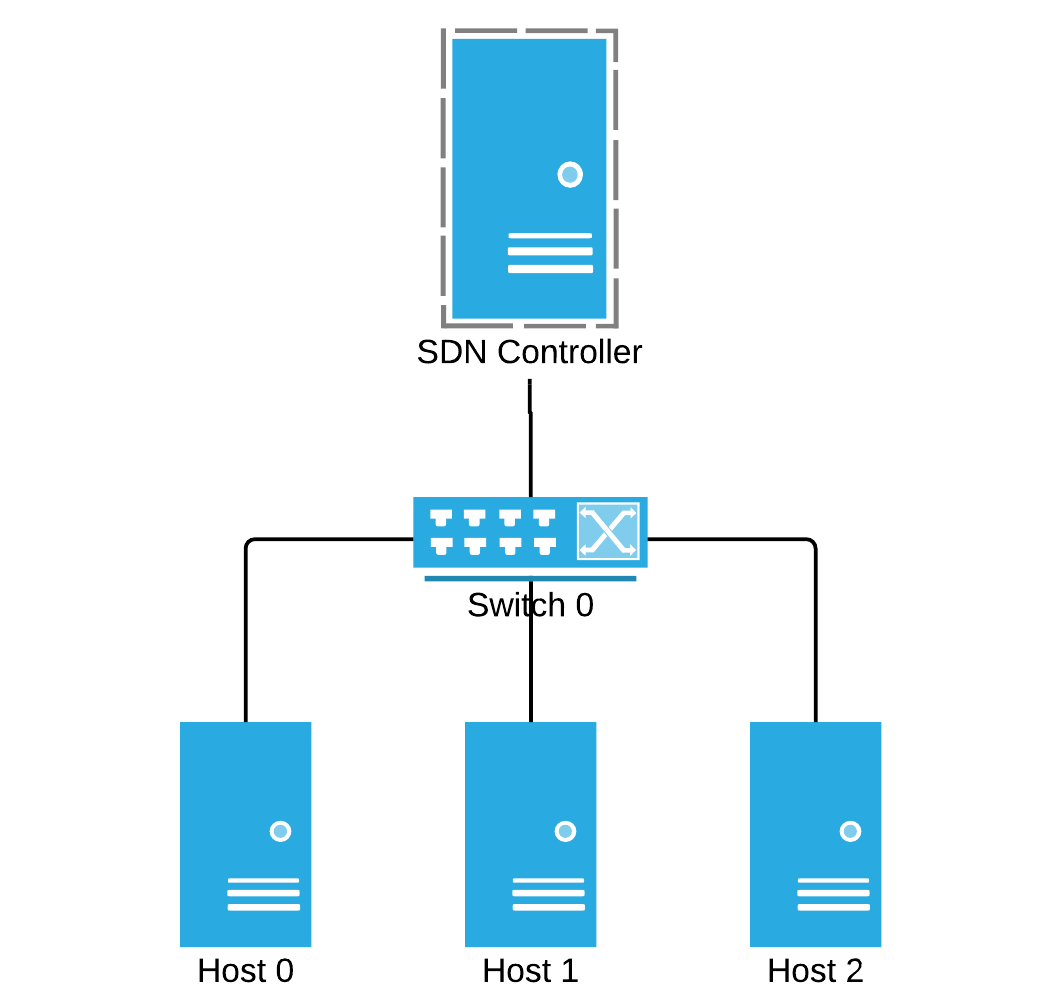
\includegraphics[scale=0.3]{images/simple-topology.png}
    \end{figure}
\end{frame}


%
% N openflow 
%
\begin{frame}\frametitle{Arquitetura Openflow}

    \begin{itemize}
    \item Um controlador para vários \emph{Switches}
    \end{itemize}
    
	\begin{figure}[h]
        \centering
        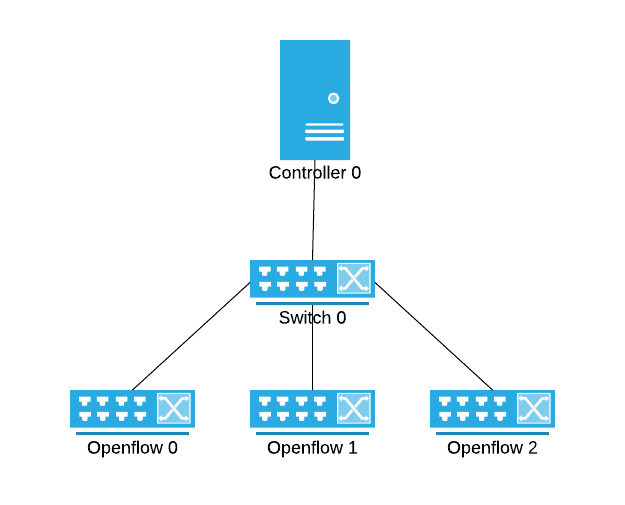
\includegraphics[scale=0.4]{images/n-openflow-switches.png}
    \end{figure}
\end{frame}


%
% SDN inter domain
%
\begin{frame}\frametitle{Arquitetura Openflow}

    \begin{itemize}
    \item Comunicação entre domínios de rede
    \end{itemize}
    
   
	\begin{figure}[h]\hspace*{-1cm}
        \centering
        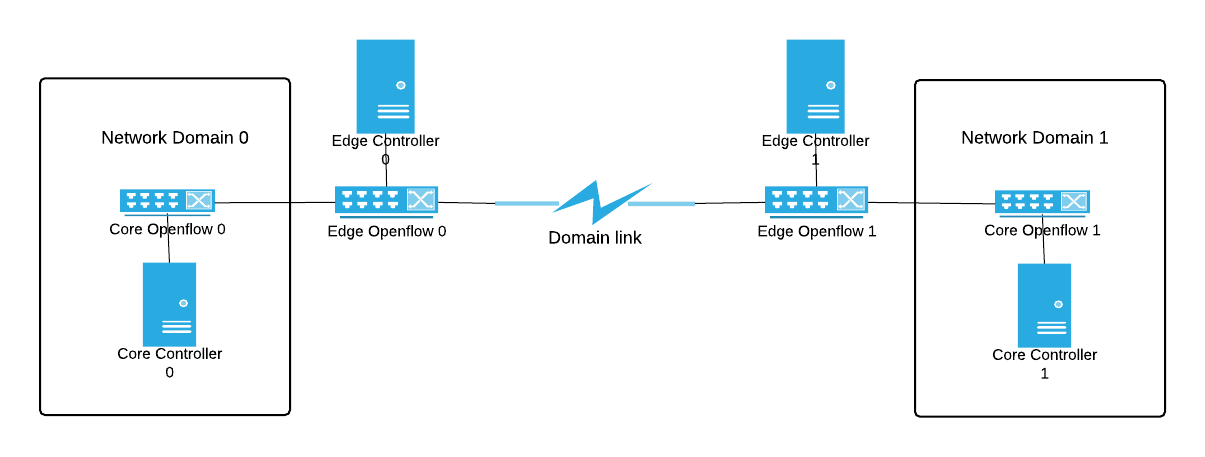
\includegraphics[scale=0.3]{images/edge-core-sdn.png}
    \end{figure}
\end{frame}



%
% Distributed openflow controller
%
\begin{frame}\frametitle{Arquitetura Openflow}

    \begin{itemize}
    \item Controlador distribuído
    \end{itemize}
    
	\begin{figure}[h]
        \centering
        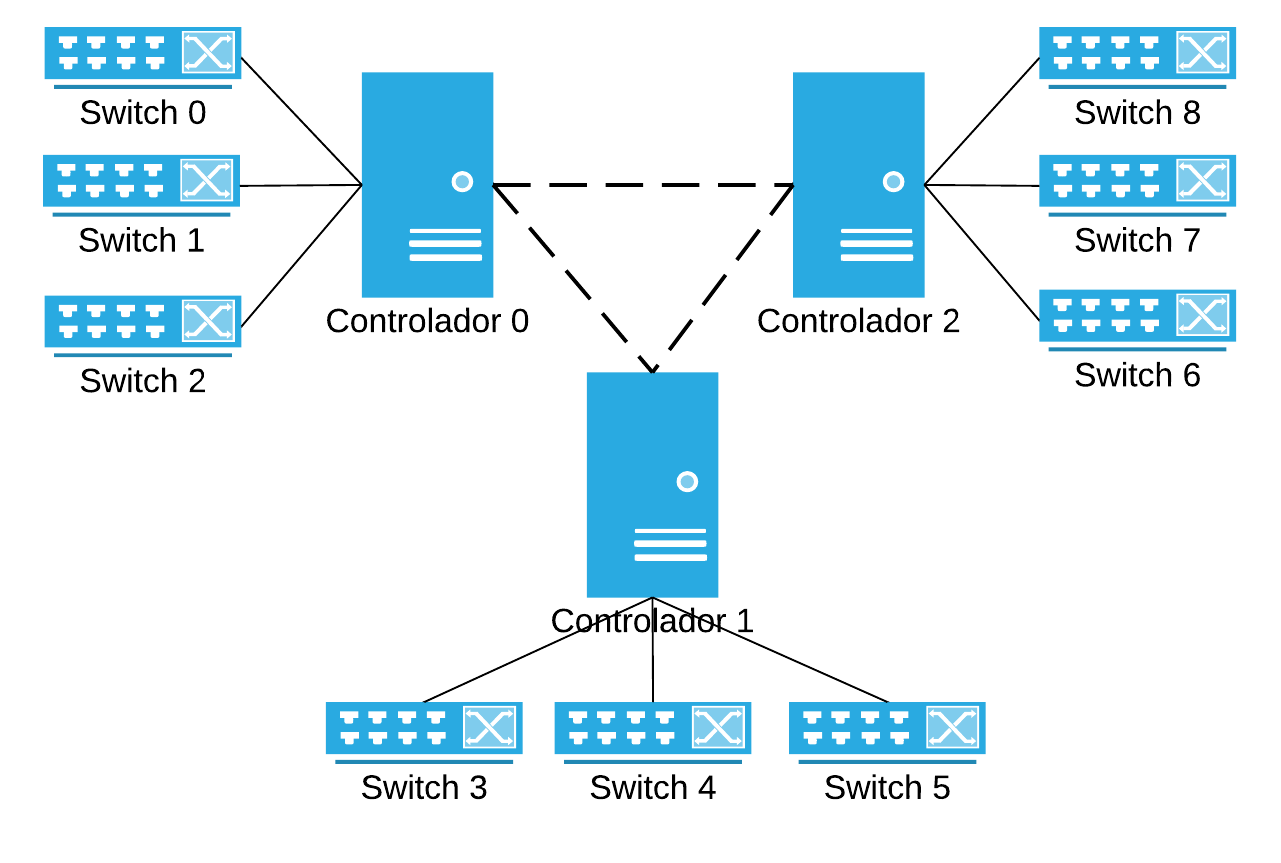
\includegraphics[scale=0.4]{images/distributed_sdn_controller.png}
    \end{figure}
\end{frame}

\chapter{Trabalhos relacionados}

Essa seção apresenta os trabalhos relacionados ao presente projeto de 
dissertação e discute suas características.
A seção segue uma linha cronológica com temas e artigos que levam a 
formulação que é a base do presente trabalho.

\section{As redes em camadas (\emph{Overlay})}

Um entendimento das implicações de redes \emph{overlays} para a 
arquitetura da Internet, para o mercado e para a política
é apresentado em \citep{clark2006overlay}. 
De modo geral o artigo descreve, principalmente, as redes de 
CDN (Redes de entrega de conteúdo), segurança e roteamento em camadas. 
O artigo posiciona as \emph{overlays} como uma uma camada intermediária, 
acima dos protocolos básicos IP e abaixo da camada de 
aplicação. 
Segundo essa visão, \emph{overlays} são para a internet básica (ponto-a-ponto)
usuários finais em que, por exemplo, um roteador apenas encaminha pacotes sem
se importar com seu conteúdo ou finalidade. 
Por outro lado, para a aplicação ela se comporta como sua infraestrutura. 
Segundo o autor, as \emph{overlays} se tornaram o principal meio de 
evolução da arquitetura da Internet.

Utilizar \emph{overlay} para tratar as deficiências da rede é custoso, no
entanto atualizar a infraestrutura da Internet básica seria ainda mais. 
As redes \emph{overlays} irão, de maneira disruptiva, representar o modo de 
inovar dentro da Internet criando novos jogadores, 
um novo cenário econômico e novas regras.

A arquitetura RON (\emph{Resilient Overlay Network}) 
\citep{anderson2001resilient} é capaz de tornar a entrega de pacotes na 
Internet mais confiável através de detecção e recuperação de interrupções e 
falhas no roteamento. 
A Internet foi criada como uma rede \emph{overlay} que funcionava sobre a rede 
de telefonia. Ou seja, o conceito de Redes \emph{overlay} não é uma idéia nova.
No entanto, poucas dessas redes foram estruturadas para se recuperar e tolerar 
falhas de forma eficiente. Nesse contexto é que as RONs demonstram ser 
confiáveis.

As RONs possuem três Metas/objetivos. O primeiro objetivo e principal é 
permitir que um grupo de nós possam se comunicar independente de haver uma 
falha na rota entre eles. 
Isso torna o roteamente confiável. O segundo objetivo
é tornar o roteamento e a seleção de próximo host com aplicações distribuídas 
mais forte, mais eficiente do que tradicionalmente é feito com outras 
arquiteturas e protocolos. 
O terceiro e último objetivo é fornecer um framework 
para implementação de políticas de roteamento que governam a escolha de rotas 
dentro da rede. 

As implicações de desempenho entre a rede \emph{overlay} Gnutella e a 
infra-estrutura da Internet é descrito em \citep{ripeanu2002mapping}. 
Redes P2P agregam vários computadores que entram e saem da rede todo o tempo. 
Esses Peers (computadores) podem não ter um endereço IP permanente. 
As redes P2P são entidades independentes e auto organizadas. 
Esse trabalho descreve um período de avaliação de sete meses do crescimento das 
redes Gnutella assim como suas implicações de desempenho. 
A rede é composta por serventes (computadores) que são os nós da rede virtual 
na camada de aplicação em que seus enlaces são formados por conexões 
TCPs abertas. 
Ao analisar a topologia utilizada pelo Gnutella o artigo explicita que apesar 
de essas redes serem eficientes em lidar com falhas aleatórias em computadores,
elas estão vulneráveis a ataques bem planejados.

\section{Redes centradas em conteúdo}

\emph{Content-Centric Networking} (CCN, redes centradas no conteúdo) trata o 
conteúdo como uma primitiva\citep{van2009networking}. 
Esse conteúdo é requisitado através de um nome. 
Em analogia ao IP, a CCN substitui o 'onde', utilizado no IP, pelo 'o que'. 
A comunicação dentro da CCN é definida por 'consumidores de dados'. 
Existem dois tipos de pacotes: \emph{Interest} (interesse) 
e \emph{Data} (dado).    

O documento descreve o funcionamento completo do roteamento dos pacotes 
baseados em conteúdo, assim como seria seu comportamento dentro de 
intra-domínios e inter-domínios. 
A segurança acontece no nível do dado ao invés de apenas uma propriedade da 
conexão pela qual o dado trafega. 
O projeto de CCN's a protege de várias classes de ataques de rede. 
O artigo apresenta comparações e avaliações de CCN's em relação ao TCP/IP. 
São relacionados temas como eficiência na tranferência de dados, 
eficiência na distribuição de conteúdo, a estratégia de camadas da rede 
e voz sobre CCN. 
A CCN foi projetada para substituir o IP, mas pode ser distribuída 
como um overlay. 

O artigo \citep{dilley2002globally} apresenta como o CDN 
(\emph{Content Delivery Network}) da Akamai's lidou com gargalos e falhas 
através de servidores de borda. 
Esses servidores são responsáveis por aliviar o serviço de estressar um único 
servidor. 
Servir conteúdo na \emph{Web} com apenas um servidor são sérios problemas 
para escalabilidade, confiança e performance de um sítio/serviço.

Ao estabelecer servidores de borda que possuem tarefas específicas, 
é necessário tratar suas falhas individulamente.
Em função dessas características, o artigo apresenta soluções com servidores de
borda através da utilização de aproximação (proxy), provisionamento (caches), 
replicação, sincronia, balanceamento de carga, tolerância a falhas, 
autenticação, segurança, recuperação de erros e monitoramento de serviços. 
O artigo propôe que o grande desafio para lidar com esses circunstâncias é 
identificar os design patterns (padrões de desenho/implementação) que são 
soluções de custo efetivo e úteis ao sistema de maneira global.


Uma experiência relevante foi a utilização do CoralCDN durante seus cinco
anos de deploy (publicação).
Com o enorme crescimento em utilizar virtualização e deploy em cloud, 
os serviços na Internet estão cada vez mais descentralizando
sua infra-estrutura. 
O CoralCDN foi desenvolvido de maneira escalável e automática para lidar com 
picos repentinos no tráfego de conteúdo \citep{freedman2010experiences}. 
O artigo demonstra a sequência de acontecimentos que ocorrem dentro da rede de 
aproximadores (proxys), servidores de índice, DNS e origem quando um cliente 
requisita uma url ao CDN. 

O CoralCDN, objetiva poupar ao máximo os servidores origem. 
A utilização de aproximadores (proxys) e provisionamento (cache) 
garantem que esse objetivo seja cumprido. 
O funcinamento interno do CDN estabelece políticas de acesso aos conteúdos. 
Diferenciando políticas para recuperar conteúdos antigos, conteúdos não 
populares, excessos para conteúdos populares e de muito acesso. O CDN 
disponibiliza também, uma API aberta para permitir elasticidade na 
distribuição de conteúdo. 

O protocolo Chord de pesquisa de itens em nós dentro de uma 
rede Peer-to-peer é aprensentado em \citep{ion2001chord}. 
O Chord executa apenas uma operação em que, dada uma chave, 
ele mapeia a chave a um nó (host). 
A tabela de roteamento Chord é distribuída e utiliza hashing para 
atribuir uma chave a um nó. 
O artigo prova que a complexidade algorítmica dessa busca é O(log N).
O Chord simplifica o modelo P2P, lidando apenas com balanceamento de carga, 
descentralização, escalabilidade, disponibilidade e nomeação flexível. 
É provado que as buscas recursivas são mais eficientes em 
função do tempo de execução do que as pesquisas iterativas. 
Diferentemente de P2Ps como Napster e Gnutella, o protocolo Chord melhora a 
escalabilidade da tarefa de embaralhamento (hashing), pois ele evita que 
todos os nós tenham que saber sobre todos os demais nós. 

ICN (Information Centric Network) \citep{bong2009information} é uma abordagem 
parecida com a CCN (Content centric Network). 
O artigo mostra uma arquitetura bem parecida com SDNs onde o plano de controle 
está separado do plano de dados. Mostra também que esses planos são unidades 
lógicas dentro da rede. Ou seja, o controlador pode ser composto por diversos 
equipamentos (entidades) na rede. 

O artigo, abstrai o funcionamento da busca de dados dentro da rede. 
Ele parte do pressuposto que a busca funcione como um DNS, dado que a busca é 
feita por pacotes que carregam os interesses de quem iniciou a requisição. 
Os switches ao longo da rede fazem cache dos pacotes de dado, podendo 
responder a requisição sozinhos. 

\section{O protocolo OpenFlow e as inovações em rede}

A evolução da Internet é uma discussão polêmica. 
O artigo \citep{jennifer2010future} apresenta dois pontos de vista.
O primeiro defende que a Internet necessita de um redesign. 
O segundo apresenta um ponto de vista contrário argumentando que a rede 
deve evoluir e não ser recontruída.

O primeiro ponto de vista levanta questionamentos como se deve-se continuar
fazendo melhorias na rede ou se contruir uma nova arquitetura seria melhor, 
dado que elas seriam irrestritas pelo atual modelo. 
É argumentado que o sucesso da atual Internet não significa que 
ela está amadurecida. 
É descrito que a rede não está preparada para os dispositivos e 
pequenos sensores, atualmente utilizados dentro da rede, que podem 
revolucionar a sociedade contemporânea.

Um contraponto é apresentado dizendo que a economia industrial moderna não 
está habilitada a receber essas tecnologias emergentes e que isso involveria 
custos inconscebíveis em mudar operação e tecnologia envolvida. 
É descrito também que os estudos de novas arquiteturas para a rede, para que 
seja aceitável, deve substituir por completo o atual modelo. 
Do contrário, seria apenas mais exercício intelectual para a contrução 
da nova rede. 

O projeto do protocolo OpenFlow foi apresentado em \citep{nick2008openflow}. 
Ele é uma forma de pesquisadores experimentarem novos protocolos nas redes 
utilizadas no dia-a-dia. Ele é baseado nos switches ethernet com uma tabela de 
fluxos e uma interface bem definida de comunicação com computadores externos. 

Os pesquisadores podem controlar seus próprios fluxos, escolhendo uma rota
alternativa para os pacotes ou executando algum processamento no pacote. 
Eles podem testar modelos de segurança, schemas de endereçamento e até 
alternativas ao protocolo IP. 
É possível fazer estudos em redes isoladas, em administração de redes, 
em controle de acesso, autenticação e processamento de pacotes.
O OpenFlow possibilita experimentações de maneira uniforme em switches 
completamente heterogeneos. 

Baseando-se em SDN, o artigo \citep{barath2012software} propõe uma arquitetura 
na linha evolucionária para Internet.
Como a arquitetura da Internet possui deficiências e possui diversos fatores
que impedem que ela seja substituída, o artigo traz uma abordagem que dissocia 
a infraestrutura da arquitetura da Internet. 

A arquitetura proposta envolve fundamentos trazidos de SDN, MPLS e 
encamimhamento via programas (\emph{software forwarding}). 
Nessa arquitetura, as redes seriam domínios. 
Cada domínio possui um controlador do núcleo (\emph{core}) e um 
de borda (\emph{edge}). 
Os controladores de borda controlam o tráfego externo. 
Os de núcleo controlam o interior dos domínios. 
Isso cria uma camada de isolamento em que pode-se alterar protocolos e 
algorítmos em ambos os ambientes, núcleo e borda, sem que um interfira 
no outro.
Além disso foram mostrados modelos de serviços que podem ser estruturados 
sobre essa arquitetura. 
O artigo apresenta três exemplos de sistemas de redes que poderiam funcionar 
perfeitamente sobre essa arquitetura.

\section{Computação em arquiteturas na nuvem (\emph{cloud})}

O artigo \citep{arsalan2009applying} apresenta o NOX 
(\emph{Networking Operanting System}). 
O NOX traz um controle lógico centralizado de alto nível de abstrações de 
rede como usuários, topologia, serviços e controle da rede. 
Através do OpenFlow ele adiciona entradas de fluxo (\emph{flow entries}) na 
tabela de encaminhamento dos switches. 

O projeto permite implementações em C++ e Python. 
A abordagem do artigo é voltada para datacenters. 
São demonstradas interações com PortLand e LV2. 
O grande objetivo desse sistema de gerenciamento é prover um controle da rede,
flexível suficiente, para atender uma ampla gama de necessidades de rede em 
datacenters. 
Pelo fato de artigo trazer uma abordagem mais comercial (\emph{datacenters}), 
são demonstradas as necessidades e problemas enfrentados por 
\emph{datacenters} e como o NOX demonstra-se uma ferramenta que flexibiliza 
e facilita o design dessas aplicações comerciais.

Visando solucionar o problema de migração de máquinas virtuais, 
o artigo \citep{erik2012live} apresentao LIME.
Ele é uma solução baseada em SDN que isola a aplicação da topologia da rede e 
de como ela é controlada. 
A proposta visa reduzir o tempo com que a migração e sincronia acontecem.

Ao iniciar uma migração de máquina virtual, os switches que estavam no local 
de origem e os do local de destino são agrupados em um único switch virtual. 
Todo o fluxo de dados é repassado ao controlador SDN que controla todo o 
tráfego durante o processo de migração. 
Concluída a migração o LIME reprograma os switches e descarta a necessidade 
do controlador SDN interferir no trafego.

Os dispositivos intermediários (\emph{middleboxes}) são parte crucial das 
grandes redes comporativas, centros de dados 
(\emph{datacenters}) e computação na nuvem (\emph{clouds}). 
Seu gerenciamento é complexo dinâmico.
O artigo \citep{aaron2012toward} apresenta a idéia de um arcabouço 
(\emph{framework}) utilizando SDN para gerenciar os dispositivos 
\emph{middleboxes}. 

O trabalho apresenta um arcabouço (\emph{framework}) que possibilita 
novas aplicações.
Com a separação do plano de dados do plano de controle através da SDN, 
tem-se maior flexibilidade para posicionar os dispositivos (\emph{middleboxes})
dentro da rede, assim como simplificar seu gerenciamento. 
São apresentados também abstrações e interfaces para lidar
com os estados dos dispositivos intermediários (\emph{middleboxes}). 
Essa tarefa não é nada trivial, pois esses dispositivos (\emph{middleboxes}) 
podem ser muito diferentes uns dos outros.

A configuração em tempo real (\emph{run-time}) de redes para 
grandes volumes de dados (\emph{big data}) com o objetivo de otimizar a 
aplicação juntamente com o desempenho e utilização da rede é apresentado
em \citep{programming2012guohui}.
O trabalho se baseia na utilização de \emph{switches} óticos como premissa 
para aumentar a performance.
A abordagem dos autores envolve um controlador SDN que é uma 
interface para as aplicações dentro do datacenter. 
O artigo foca bastante na topologia física e no roteamento de 
aplicações em \emph{big data}.
Ao utilizar um controlador SDN, as aplicações em \emph{big data} tornam-se 
mais próximas à rede que está abaixo da aplicação. 
O artigo utiliza o \emph{Hadoop} como exemplo de testes. São discutidos 
aspectos de integração de rede, agendamento de tarefas, topologia e 
configuração de rotas para processos \emph{Hadoop}. 


\section{Recuperação de informação topológica}

A necessidade de se buscar e monitorar dados 
específicos, principalmente em redes complexas, atrai o desenvolvimento
de linguagens DSL (linguagens de domínio especifico) que simplifique, 
organize, generalize e garanta eficiência na manipulação desses dados.
Esse é o exemplo do Frenetic \citep{foster2011frenetic} 
e do Pyretic \citep{monsanto2013composing}.

O Pyretic introduz novas abstrações para criação de aplicações de vários
módulos independentes, que em juntos administram o tráfego e 
abstraem a topologia da rede. 
O sistema utiliza uma linguagem chamada Pyretic \citep{monsanto2013composing}. 
O sistema funciona em cima do POX. 
Ele converte regras de plano de controle programadas em Pyretc para o plano 
de dados dos dispositivos de rede dentro de um SDN. 
O artigo apresenta o conjunto de regras de composição como regras de ação, 
regras de predicado, regras de consulta, etc. 
O Pyretic é uma linguagem que permite programadores a criarem grandes e 
sofisticadas aplicações SDN com pequenos módulos independentes. 

Enquanto a abordagem da DSL é baseada em atuação, execução,
conjunta com o controlador,
o NIB é baseada em um banco de dados distribuído,
com uma abordagem mais ampla e atacando problemas mais gerais
como persistência, concorrência, redundância, escalabilidade, etc.

\section{A abordagem em grafos}

A abordagem de representar a rede na forma de um grafo foi mencionada 
por Casado \emph{et al.} em um dos primeiros artigos sobre SDN
\citep{martin2010virtualizing}.
No entanto, nenhum detalhe de implementação é apresentado.
Em um trabalho futuro, uma solução SDN foi desenvolvida através de 
diferentes topologias de rede dentro do contexto de \emph{datacenter} 
em que a abstração em grafos não foi adotada \citep{ripcord}. 

Raghavendra \emph{et al.} apresenta um módulo em grafos com capacidade 
de atualização dinâmica com uma API para algorítmos em grafos
\citep{ramya2012dynamic}.
Esse trabalho não possui nenhuma integração com algum controlador SDN,
que é a base da avaliação do presente trabalho.

O controlador \emph{Onix} \citep{teemu2010onix} foi projetado em torno do 
conceito NIB (\emph{Network Information Base}), que é uma base 
de informações da rede.
Essa base mantém uma visão global da rede de maneira similar à 
MIB (\emph{Management Information Base}) implementada sobre o
protocolo SNMP.
Essa representação baseada em grafos é alcançada indexando cada
entrada de elemento em relação a seus vizinhos.





% Bibliograph file
\ppgccbibliography{src/references}


%\input{apendice} % ARQUIVO CONTENDO OS APÊNDICES : OPCIONAL
%\input{anexo} % ARQUIVO CONTENDO OS ANEXOS: OPCIONAL

\end{document}
